% Options for packages loaded elsewhere
% Options for packages loaded elsewhere
\PassOptionsToPackage{unicode}{hyperref}
\PassOptionsToPackage{hyphens}{url}
\PassOptionsToPackage{dvipsnames,svgnames,x11names}{xcolor}
%
\documentclass[
  11pt,
]{article}
\usepackage{xcolor}
\usepackage[margin=1in]{geometry}
\usepackage{amsmath,amssymb}
\setcounter{secnumdepth}{5}
\usepackage{iftex}
\ifPDFTeX
  \usepackage[T1]{fontenc}
  \usepackage[utf8]{inputenc}
  \usepackage{textcomp} % provide euro and other symbols
\else % if luatex or xetex
  \usepackage{unicode-math} % this also loads fontspec
  \defaultfontfeatures{Scale=MatchLowercase}
  \defaultfontfeatures[\rmfamily]{Ligatures=TeX,Scale=1}
\fi
\usepackage{lmodern}
\ifPDFTeX\else
  % xetex/luatex font selection
\fi
% Use upquote if available, for straight quotes in verbatim environments
\IfFileExists{upquote.sty}{\usepackage{upquote}}{}
\IfFileExists{microtype.sty}{% use microtype if available
  \usepackage[]{microtype}
  \UseMicrotypeSet[protrusion]{basicmath} % disable protrusion for tt fonts
}{}
\usepackage{setspace}
\makeatletter
\@ifundefined{KOMAClassName}{% if non-KOMA class
  \IfFileExists{parskip.sty}{%
    \usepackage{parskip}
  }{% else
    \setlength{\parindent}{0pt}
    \setlength{\parskip}{6pt plus 2pt minus 1pt}}
}{% if KOMA class
  \KOMAoptions{parskip=half}}
\makeatother
% Make \paragraph and \subparagraph free-standing
\makeatletter
\ifx\paragraph\undefined\else
  \let\oldparagraph\paragraph
  \renewcommand{\paragraph}{
    \@ifstar
      \xxxParagraphStar
      \xxxParagraphNoStar
  }
  \newcommand{\xxxParagraphStar}[1]{\oldparagraph*{#1}\mbox{}}
  \newcommand{\xxxParagraphNoStar}[1]{\oldparagraph{#1}\mbox{}}
\fi
\ifx\subparagraph\undefined\else
  \let\oldsubparagraph\subparagraph
  \renewcommand{\subparagraph}{
    \@ifstar
      \xxxSubParagraphStar
      \xxxSubParagraphNoStar
  }
  \newcommand{\xxxSubParagraphStar}[1]{\oldsubparagraph*{#1}\mbox{}}
  \newcommand{\xxxSubParagraphNoStar}[1]{\oldsubparagraph{#1}\mbox{}}
\fi
\makeatother


\usepackage{longtable,booktabs,array}
\usepackage{calc} % for calculating minipage widths
% Correct order of tables after \paragraph or \subparagraph
\usepackage{etoolbox}
\makeatletter
\patchcmd\longtable{\par}{\if@noskipsec\mbox{}\fi\par}{}{}
\makeatother
% Allow footnotes in longtable head/foot
\IfFileExists{footnotehyper.sty}{\usepackage{footnotehyper}}{\usepackage{footnote}}
\makesavenoteenv{longtable}
\usepackage{graphicx}
\makeatletter
\newsavebox\pandoc@box
\newcommand*\pandocbounded[1]{% scales image to fit in text height/width
  \sbox\pandoc@box{#1}%
  \Gscale@div\@tempa{\textheight}{\dimexpr\ht\pandoc@box+\dp\pandoc@box\relax}%
  \Gscale@div\@tempb{\linewidth}{\wd\pandoc@box}%
  \ifdim\@tempb\p@<\@tempa\p@\let\@tempa\@tempb\fi% select the smaller of both
  \ifdim\@tempa\p@<\p@\scalebox{\@tempa}{\usebox\pandoc@box}%
  \else\usebox{\pandoc@box}%
  \fi%
}
% Set default figure placement to htbp
\def\fps@figure{htbp}
\makeatother





\setlength{\emergencystretch}{3em} % prevent overfull lines

\providecommand{\tightlist}{%
  \setlength{\itemsep}{0pt}\setlength{\parskip}{0pt}}



 
\usepackage[]{biblatex}
\addbibresource{references.bib}


\usepackage{hyperref}
\hypersetup{
  colorlinks=true,
  linkcolor=blue,
  urlcolor=blue,
  breaklinks=true,
  pdfborder={0 0 0}
}
\makeatletter
\@ifpackageloaded{caption}{}{\usepackage{caption}}
\AtBeginDocument{%
\ifdefined\contentsname
  \renewcommand*\contentsname{Table of contents}
\else
  \newcommand\contentsname{Table of contents}
\fi
\ifdefined\listfigurename
  \renewcommand*\listfigurename{List of Figures}
\else
  \newcommand\listfigurename{List of Figures}
\fi
\ifdefined\listtablename
  \renewcommand*\listtablename{List of Tables}
\else
  \newcommand\listtablename{List of Tables}
\fi
\ifdefined\figurename
  \renewcommand*\figurename{Figure}
\else
  \newcommand\figurename{Figure}
\fi
\ifdefined\tablename
  \renewcommand*\tablename{Table}
\else
  \newcommand\tablename{Table}
\fi
}
\@ifpackageloaded{float}{}{\usepackage{float}}
\floatstyle{ruled}
\@ifundefined{c@chapter}{\newfloat{codelisting}{h}{lop}}{\newfloat{codelisting}{h}{lop}[chapter]}
\floatname{codelisting}{Listing}
\newcommand*\listoflistings{\listof{codelisting}{List of Listings}}
\makeatother
\makeatletter
\makeatother
\makeatletter
\@ifpackageloaded{caption}{}{\usepackage{caption}}
\@ifpackageloaded{subcaption}{}{\usepackage{subcaption}}
\makeatother
\usepackage{bookmark}
\IfFileExists{xurl.sty}{\usepackage{xurl}}{} % add URL line breaks if available
\urlstyle{same}
\hypersetup{
  pdftitle={William's Update},
  pdfauthor={William Clinton Co},
  colorlinks=true,
  linkcolor={blue},
  filecolor={Maroon},
  citecolor={blue},
  urlcolor={blue},
  pdfcreator={LaTeX via pandoc}}


\title{William's Update}
\usepackage{etoolbox}
\makeatletter
\providecommand{\subtitle}[1]{% add subtitle to \maketitle
  \apptocmd{\@title}{\par {\large #1 \par}}{}{}
}
\makeatother
\subtitle{Case Study and Data}
\author{William Clinton Co}
\date{July 24, 2025}
\begin{document}
\maketitle
\begin{abstract}
This paper provides an exploratory update in support of the research
agenda ``Productivity and Wedges: Economic Convergence and the Real
Exchange Rate'' (Devereux, Fujiwara, \& Granados, 2025). It evaluates
the possibility of applying a Korea-style case study framework,
highlighting structural transformation, independent monetary regimes,
and convergence---to selected European Union (EU) economies. We identify
datasets on real exchange rates and inflation targeting frameworks using
sources such as Eurostat, the IMF (Zhang, 2025), and BIS (Chavaz, 2025).
We also assess candidate countries for case study analysis, with
particular focus on Estonia, Ireland, Slovakia, and Poland. Estonia and
Slovakia are identified as the most promising analogues to Korea, given
their respective strengths in technology and automotive exports.
\end{abstract}

\renewcommand*\contentsname{Table of contents}
{
\hypersetup{linkcolor=}
\setcounter{tocdepth}{3}
\tableofcontents
}

\setstretch{1}
\section{Introduction}\label{introduction}

This document presents an exploratory update to support the development
of a case study and data for a research project inspired by
\emph{``Productivity and Wedges: Economic Convergence and the Real
Exchange Rate''} (Devereux, Fujiwara, \& Granados, 2025). In particular,
it considers whether a case study approach similar to that of
\href{https://www.nber.org/system/files/working_papers/w32769/w32769.pdf}{Irwin
and Obstfeld (2024)}, which focused on Korea's structural reforms,
currency regime, and convergence, can be applied to selected European
Union (EU) member states.

We also identify datasets on real exchange rates (RER) and monetary
policy frameworks and evaluate possible case study candidates among EU
countries. Another goal is to identify economies with comparable
dynamics to Korea, particularly in relation to structural
transformation, tradable sector development, and macroeconomic
convergence.

This document includes:

\begin{itemize}
\tightlist
\item
  Identified datasets on real exchange rates and monetary policy targets
  data\\
\item
  An overview of potential EU case studies\\
\item
  Comparative analysis of Estonia, Slovakia, Ireland, Poland, and others
\end{itemize}

\section{Data Update}\label{data-update}

\subsection{European Currency Data}\label{european-currency-data}

We now have a dataset sourced from \textbf{Eurostat} that contains the
\textbf{real exchange rates} of European Union countries.

\textbf{Dataset details:}

\begin{itemize}
\tightlist
\item
  \textbf{Time period:} Annual data from \textbf{2000 to 2021}
\item
  \textbf{Scope:} Exchange rates are \textbf{relative to other EU
  countries}
\item
  \textbf{Countries included:} Limited to those discussed, all of which
  are EU members (or closely aligned)
\end{itemize}

\textbf{Relevant currencies:}

\begin{itemize}
\tightlist
\item
  \textbf{BGN} -- Bulgarian Lev \emph{(Bulgaria)}
\item
  \textbf{CZK} -- Czech Koruna \emph{(Czech Republic)}
\item
  \textbf{DKK} -- Danish Krone \emph{(Denmark)}
\item
  \textbf{HUF} -- Hungarian Forint \emph{(Hungary)}
\item
  \textbf{PLN} -- Polish Zloty \emph{(Poland)}
\item
  \textbf{RON} -- Romanian Leu \emph{(Romania)}
\item
  \textbf{SEK} -- Swedish Krona \emph{(Sweden)}
\end{itemize}

\textbf{Link to dataset:}

\begin{itemize}
\tightlist
\item
  \href{https://ec.europa.eu/eurostat/databrowser/view/ert_bil_eur_a/default/table?lang=en}{Eurostat:
  Real Exchange Rates (Annual)}
\item
  \href{https://github.com/WilliamClintC/RER/tree/main/data/Eurostat/estat_ert_bil_eur_a_en.csv}{Github}
\end{itemize}

\subsection{Monetary Policy Dataset}\label{monetary-policy-dataset}

There are two key datasets relevant for analyzing monetary policy
frameworks in our study:

\subsubsection{Zhongxia Zhang (IMF,
2025)}\label{zhongxia-zhang-imf-2025}

This dataset provides detailed information on inflation targeting
regimes, including:

\begin{itemize}
\tightlist
\item
  \textbf{Inflation targets and bands}
\item
  \textbf{Track records of target adherence}
\end{itemize}

The dataset is available via:

\begin{itemize}
\tightlist
\item
  \href{https://data.mendeley.com/datasets/g9m7rnvtw7/2?utm_source}{Mendeley
  Data (Zhang 2025)}
\item
  \href{https://github.com/WilliamClintC/RER/blob/main/data/Inflation\%20Targeting\%20Dataset\%20Inflation\%20Targets\%2C\%20Bands\%2C\%20and\%20Track\%20Records/Inflation\%20targeting\%20dataset_Zhang\%202025\%20May\%20online\%20version.xlsx}{GitHub
  Repository}
\end{itemize}

This dataset is ideal for capturing \textbf{explicit inflation target
levels}, \textbf{tolerance bands}, and the \textbf{credibility/track
record} of central banks over time.

\subsubsection{Boris Chavaz (2025)}\label{boris-chavaz-2025}

The Chavaz dataset offers a complementary view by detailing:

\begin{itemize}
\tightlist
\item
  \textbf{Target horizons}
\item
  \textbf{Central bank objectives beyond inflation}, including:

  \begin{itemize}
  \tightlist
  \item
    Real economy
  \item
    Financial stability
  \end{itemize}
\item
  \textbf{Relative weightings assigned to each objective}
\end{itemize}

These weights help us understand whether price stability is the dominant
concern or part of a broader set of macroeconomic goals.

\begin{itemize}
\tightlist
\item
  \href{https://github.com/WilliamClintC/RER/blob/main/data/Inflation\%20Targeting\%20Dataset\%20Inflation\%20Targets\%2C\%20Bands\%2C\%20and\%20Track\%20Records/qt2503c_online_dataset.xlsx}{BIS
  Dataset -- Chavaz (2025)}
\item
  \href{https://www.bis.org/publ/qtrpdf/r_qt2503c.htm?}{BIS Publication
  Overview}
\end{itemize}

An infographic chart that summarizes central bank objectives and their
weights, such as numerical targets, horizons, and deviations from strict
price stability

\begin{figure}[H]

{\centering \pandocbounded{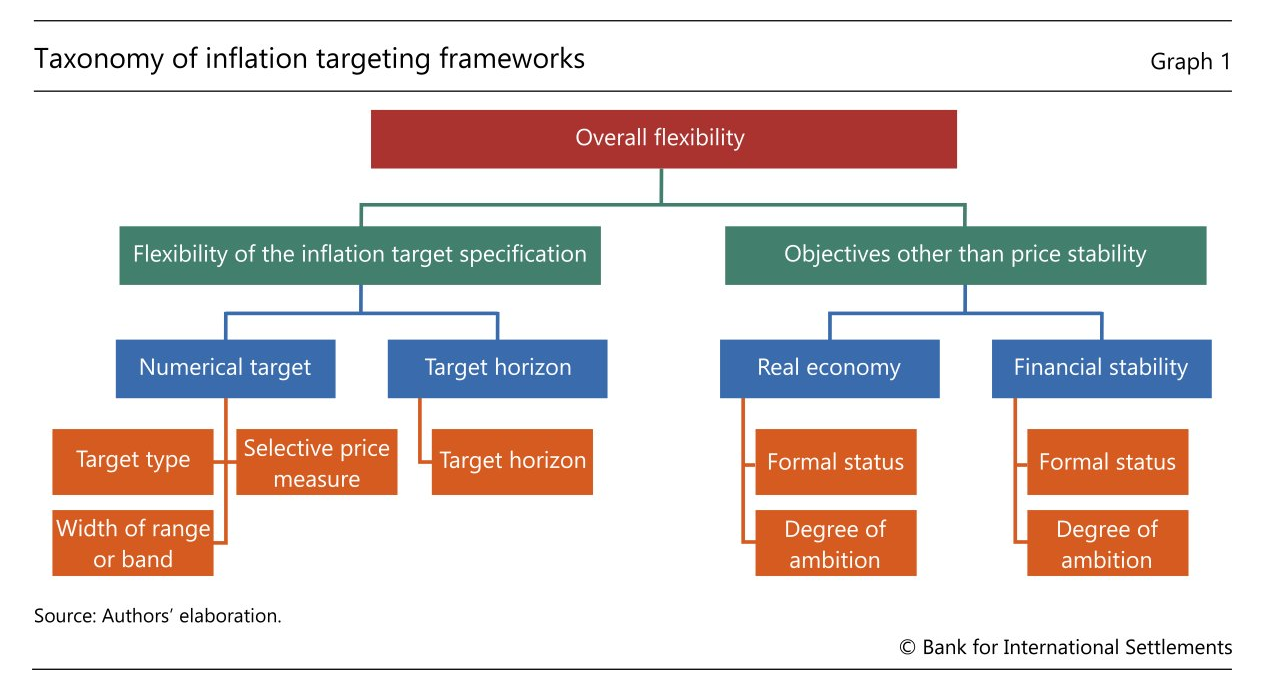
\includegraphics[keepaspectratio]{data/Inflation Targeting Dataset Inflation Targets, Bands, and Track Records/Screenshot 2025-07-24 040943.png}}

}

\caption{Central bank objectives and weights}

\end{figure}%

These two datasets, when used together, allow us to assess both the
\textbf{explicit inflation targeting frameworks} and the \textbf{broader
monetary policy record} across countries.

\section{Case Study}\label{case-study}

We investigated whether a case study, inspired by the approach of
Douglas A. Irwin and Maurice Obstfeld (2024)
{[}\href{https://www.nber.org/papers/w32769}{LINK}{]}, which focused on
Korea, could be implemented similarly for our research.

To do this, we examined the aspects of their paper that made Korea a
particularly compelling case. Notably, Korea experienced:

\begin{itemize}
\tightlist
\item
  Rapid growth in its tradable sector\\
\item
  The presence of an independent currency\\
\item
  Accelerated economic convergence
\end{itemize}

These characteristics made Korea an ideal candidate for analyzing real
exchange rate dynamics and structural transformation.

To identify analogous cases within the European Union, we looked for
countries exhibiting similar trends, especially rapid expansion of the
tradable sector, structural reforms, and substantial convergence.

\subsection{Ireland}\label{ireland}

Ireland emerged as a potential case due to the ``Celtic Tiger'' era
during the 1990s, marked by:

\begin{itemize}
\tightlist
\item
  Rapid expansion in the tradable sector, particularly in technology and
  pharmaceuticals\\
\item
  Significant foreign direct investment and export-led growth
\end{itemize}

However, a major limitation of using Ireland is its status as a
financial and corporate tax haven. This distorts national accounts data
due to profit-shifting and accounting practices of multinationals,
potentially biasing observations.

\subsection{Estonia}\label{estonia}

Estonia is a strong candidate, with:

\begin{itemize}
\tightlist
\item
  Remarkable productivity growth\\
\item
  Rapid development in technology sector\\
\item
  Rapid convergence of export tradables since its post-Soviet transition
\item
  Inolved in EU and had independent currency
\item
  Ties to former Soviet Union
\end{itemize}

Estonia has the highest number of technology unicorns per capita in the
world. Notable companies include \textbf{Skype}, \textbf{Bolt}, and
\textbf{Wise}.

\pandocbounded{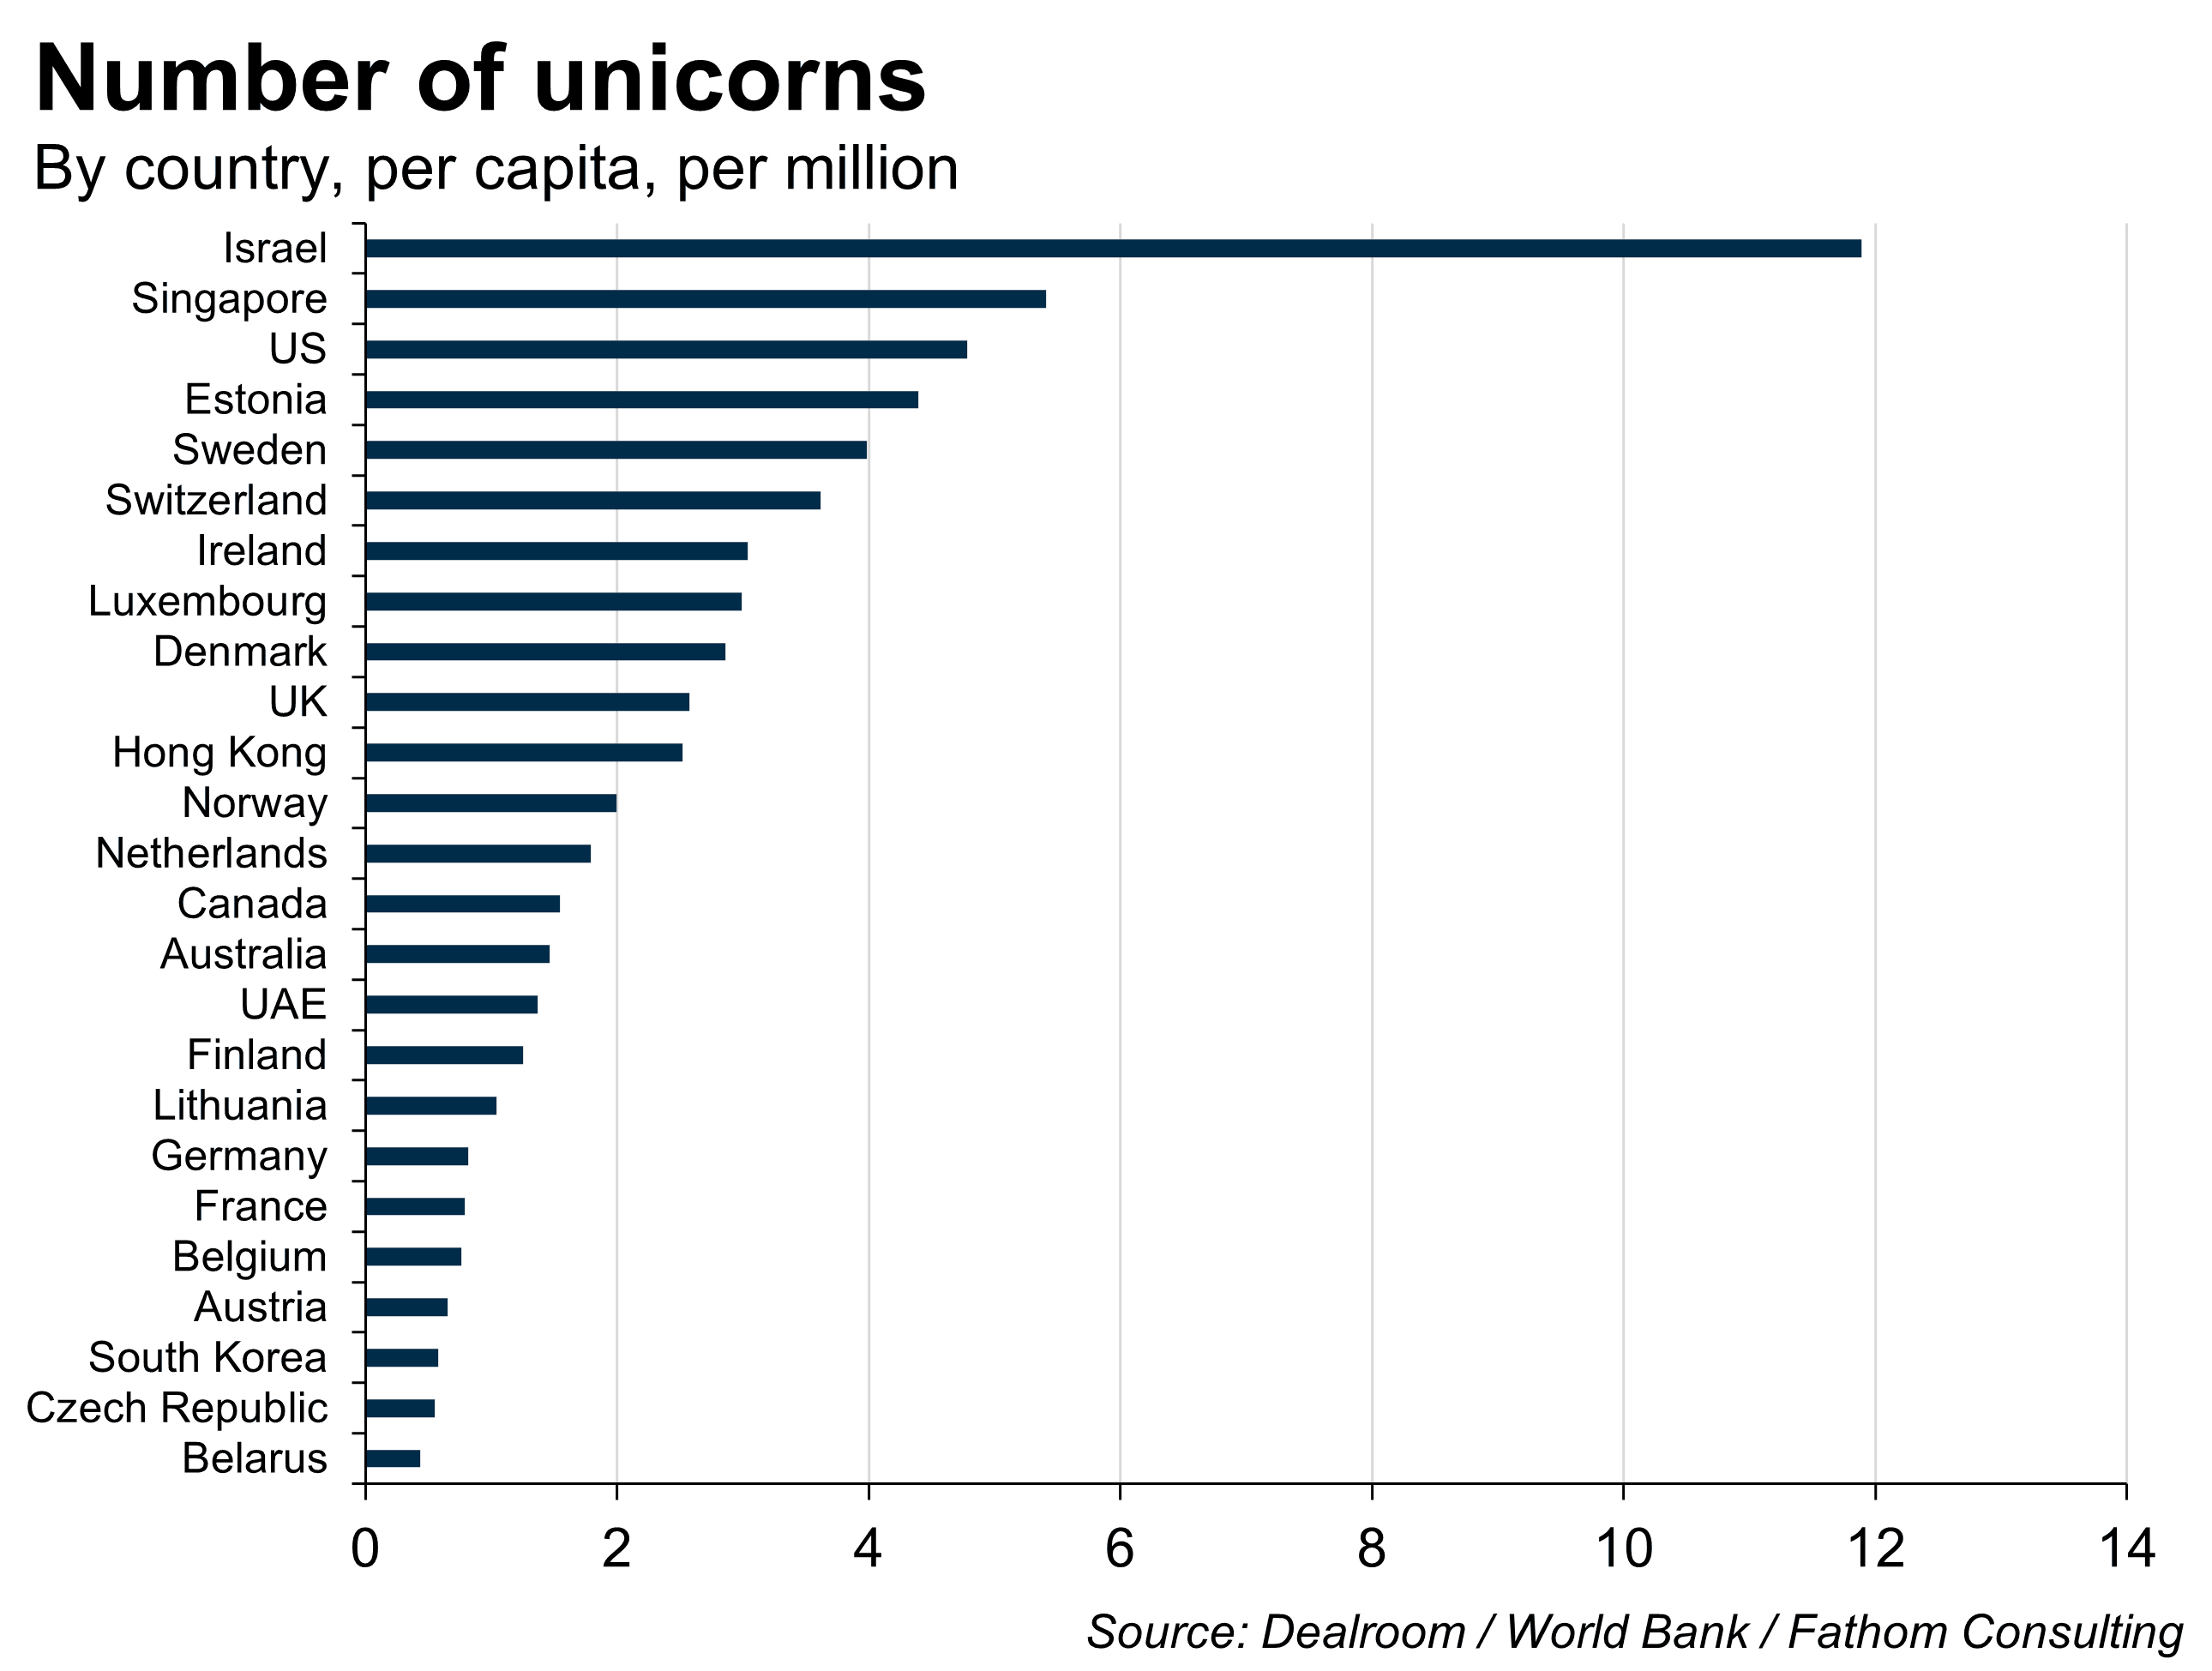
\includegraphics[keepaspectratio]{data/Inflation Targeting Dataset Inflation Targets, Bands, and Track Records/Chart-3.png}}

Estonia joined the European Union in 2004 and adopted the euro in 2011.
Its economy is highly open, with exports comprising over 80\% of GDP.
Like Korea, Estonia implemented deep structural reforms during a period
of economic crisis, making it a relevant comparison case.

Historically, Estonia's economy under Soviet rule was centered on oil
shale processing and supplying energy to the Soviet Union. Following
independence, Estonia embarked on an ambitious path of economic
modernization and integration with Western Europe, aiming to catch up
with fellow Nordic countries such as Finland.

A pivotal moment was the \textbf{Tiger Leap} initiative launched in
1996, which prioritized investment in internet access and human capital.
As a result, Estonia developed exceptional digital infrastructure, with
both the public and private sectors embracing digital technologies.
Today, Estonia is known for its fully digital government and is a global
leader in e-governance.

One limitation, however, is its small economic size relative to other EU
economies, which may affect the generalizability of findings.

\subsection{Slovakia}\label{slovakia}

Slovakia may be a strong candidate for analysis due to its strong
automotive export sector.

\pandocbounded{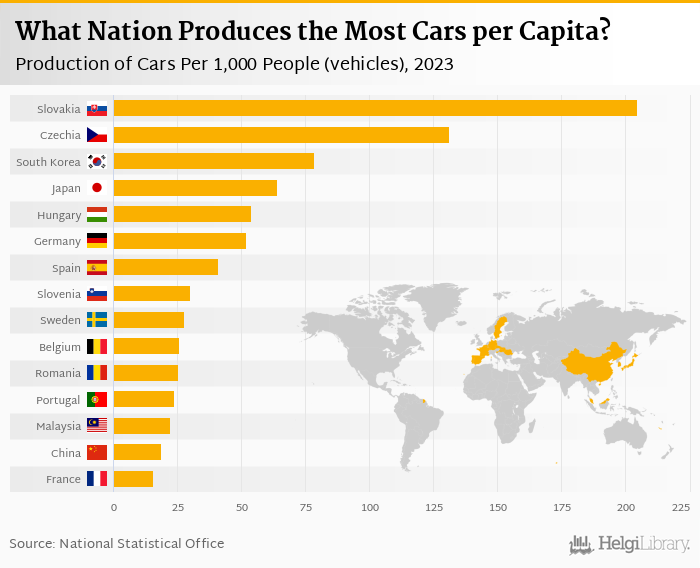
\includegraphics[keepaspectratio]{data/Inflation Targeting Dataset Inflation Targets, Bands, and Track Records/Helgi Library - What Nation Produces the Most Cars per Capita.png}}

While Estonia lacks a robust automotive industry, and Slovakia does not
have a notable technology sector, Korea stands out for having both.

Given this, it may be worth exploring a combined case study using both
Estonia and Slovakia as a composite benchmark. By examining their
complementary strengths, technology in Estonia and automotive exports in
Slovakia, we can construct a useful comparison to Korea and assess
whether similar structural dynamics are at play.

\subsection{Poland}\label{poland}

Poland is a large and rapidly growing economy but lacks standout
statistics like Slovakia's high number of cars per capita or Estonia's
high number of unicorns per capita

Poland is:

\begin{itemize}
\tightlist
\item
  The largest post-communist economy in the European Union\\
\item
  A major recipient of EU cohesion funds\\
\item
  A country that has experienced remarkable and sustained economic
  growth since its transition
\end{itemize}

However, compared to countries like Korea, with globally recognized
technology giants such as Samsung. Poland does not have a similarly
distinctive anchor, which may limit our case study.

\subsection{Other Countries
Considered}\label{other-countries-considered}

Hungary, the Czech Republic, and Spain were also evaluated as potential
case study candidates. However, they were determined less suitable due
to the absence of distinctive sectoral developments relative to the
previous countries mentioned.

\section{Closing Thoughts}\label{closing-thoughts}

It would be helpful to examine the most recent data on the convergence
of real exchange rates RER and GDP among the 12 countries considered in
the meeting last July 17, 2025. Such could offer additional insights.

\begin{center}\rule{0.5\linewidth}{0.5pt}\end{center}


\printbibliography



\end{document}
